\NeedsTeXFormat{LaTeX2e}
\documentclass[12pt,oneside,a4paper]{article}
\usepackage[left=2cm, right=2cm, top=1cm, bottom=2cm]{geometry}
\usepackage{amsmath,amsfonts,amssymb,amsthm}
\usepackage[utf8]{vietnam}
\usepackage{graphicx}
\usepackage{float}
\usepackage{mathptmx}
\usepackage{multicol}
\usepackage{enumitem} 
\usepackage{tasks} 
\usepackage{booktabs}
\usepackage{caption}
\usepackage{hyperref}

\everymath{\displaystyle}
\theoremstyle{definition}
\newtheorem{bt}{} 
\renewcommand{\thebt}{\textbf{\large Q\arabic{bt}}} 

\newcommand{\bb}[1]{\mathbb{#1}}

\newlist{questions}{enumerate}{1}
\setlist[questions]{label=\textbf{Q$_{\mathbf{\arabic*}}$:}, leftmargin=4em}

\settasks{label=\textbf{\Alph*.}, label-width=1.5em, item-indent=7mm}

\begin{document}
	\renewcommand{\figurename}{Figure}
	\renewcommand{\tablename}{Table}
	
	\begin{center}
		\textbf{\Large EXPERIMENT 4}
		
		\vspace{0.5cm}
		\textbf{\Large VERIFICATION OF FARADAY'S LAW OF}
		
		\vspace{0.1cm}
		\textbf{{\Large ELECTROMAGNETIC INDUCTION}}
	\end{center}
	
	\vspace{0.5cm}
	
	\noindent
	\begin{minipage}[t]{0.5\textwidth}
		\vspace{0.5cm}
		\textbf{Class: IT-E10 02} \\[0.2cm]
		\textbf{Group: 3} \\[0.2cm]
		\textbf{Name: Nguyễn Trọng Phúc Anh} \\[0.2cm]
		\textbf{Student ID: 202516522}
	\end{minipage}%
	\begin{minipage}[t]{0.5\textwidth}
		\vspace{0pt}
		\centering
		\textit{\textbf{Verification of the instructors}} \\[0.2cm]
		\begin{tabular}{|p{3.5cm}|p{3.5cm}|}
			\hline
			& \\[2.5cm]
			\hline
		\end{tabular}
	\end{minipage}
	
	\vspace{0.8cm}
	\section*{1. THEORETICAL BACKGROUND}
	\qquad Michael Faraday was the first scientist to find that electricity can be produced from magnetism. He discovered that when a magnet is moving relative to a coil consisting of a number of turns of conductive wire, there will be a voltage across the coil of wire as a result. The essence of his discovery is described in the following statement
	
	\textit{\textbf{A voltage is induced in a circuit whenever relative motion exists between a conductor and a magnetic field, and the magnitude of this voltage is proportional to the rate of change of the flux}}.
	\begin{equation}
		V_{\text{induced}} = -N \frac{\Delta \Phi}{\Delta t} = -N \frac{\Delta(BA)}{\Delta t}
	\end{equation}
	where $N$ is the number of wire's turns, $A$ is the cross-section area of the coil, and $\Delta \Phi$ is the change in magnetic flux resulting from the change in magnetic field $\Delta B$.
	
	Because electricity is induced by a changing magnetic field, this process is called electromagnetic induction. Faraday also realized several factors that determine how much voltage is induced: the strength of the magnetic field, how fast the magnetic field changes, and the number of turns (loops) of wire in the coil.
	
	\section*{2. EXPERIMENTAL PROCEDURE}
	
	\subsection*{2.1. Preparation of measurement}
	\begin{itemize}[leftmargin=1.5em]
		\item Turn on the SW 750 interface device and the computer.
		\item Plug a voltage sensor into channel A (or B) of Science Workshop 750 and connect it to the coil terminals.
		\item Launch Data Studio program, drag and drop "Voltage sensor" to channel A, set measurement regime as "Medium" and frequency as 500 Hz.
		\item Place a protective pad or cushion underneath the coil to catch the bar magnet after it falls through.
		\item Prepare two data tables for the 1200-turn and 150-turn coils. Each table has 3 columns: \textit{"Magnet's pole"}, \textit{"Voltage peak 1 (mV)"}, and \textit{"Voltage peak 2 (mV)"}.
	\end{itemize}
	
	\subsection*{2.2. Measurement consequences}
	\subsubsection*{2.2.1. 1200-turn coil}
	\begin{enumerate}[leftmargin=1.5em]
		\item Hold the bar magnet above the 1200-turn coil with the 'North - N' end at the bottom.
		\item Press "Start" on Data Studio interface, release the bar magnet to drop freely through the center of the coil, then press "Stop".
		\item Drag file $\text{Run}^\#1$ to "Graph" to display the induced voltage pulse.
		\item Use the "Point" tool to determine Voltage Peak 1 and Voltage Peak 2. Record values in the table and store the graph.
		\item Reverse the bar magnet so the 'South - S' end falls through first, and repeat the procedure.
		\item Tape two bar magnets together so each end has a combined 'north' and 'south' pole, and repeat the measurement.
		\item Rearrange the two bar magnets so one end is 'north-north' and the other is 'south-south', and repeat the measurement.
	\end{enumerate}
	
	\subsubsection*{2.2.2. 150-turn coil}
		Repeat the measurement procedure similarly for the 150-turn coil using single and double bar magnets, and record results in the second data table.
	
	\section*{3. EXPERIMENTAL RESULTS}
	
	\subsection*{3.1. 1200-turn coil}
	\subsubsection*{3.1.1. Graph}
	\begin{center}
		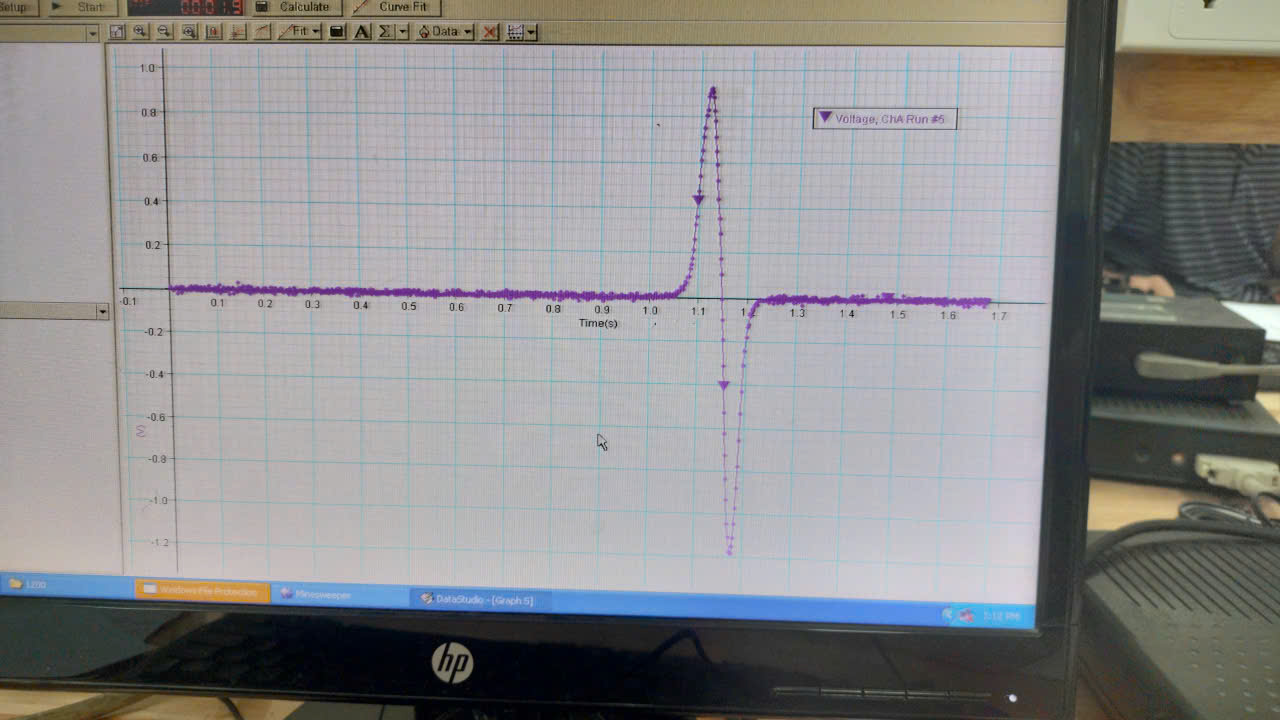
\includegraphics[width=0.95\textwidth]{1200 N.jpg}
		\captionof{figure}{\textit{North-pole down}}
	\end{center}
	
	\begin{center}
		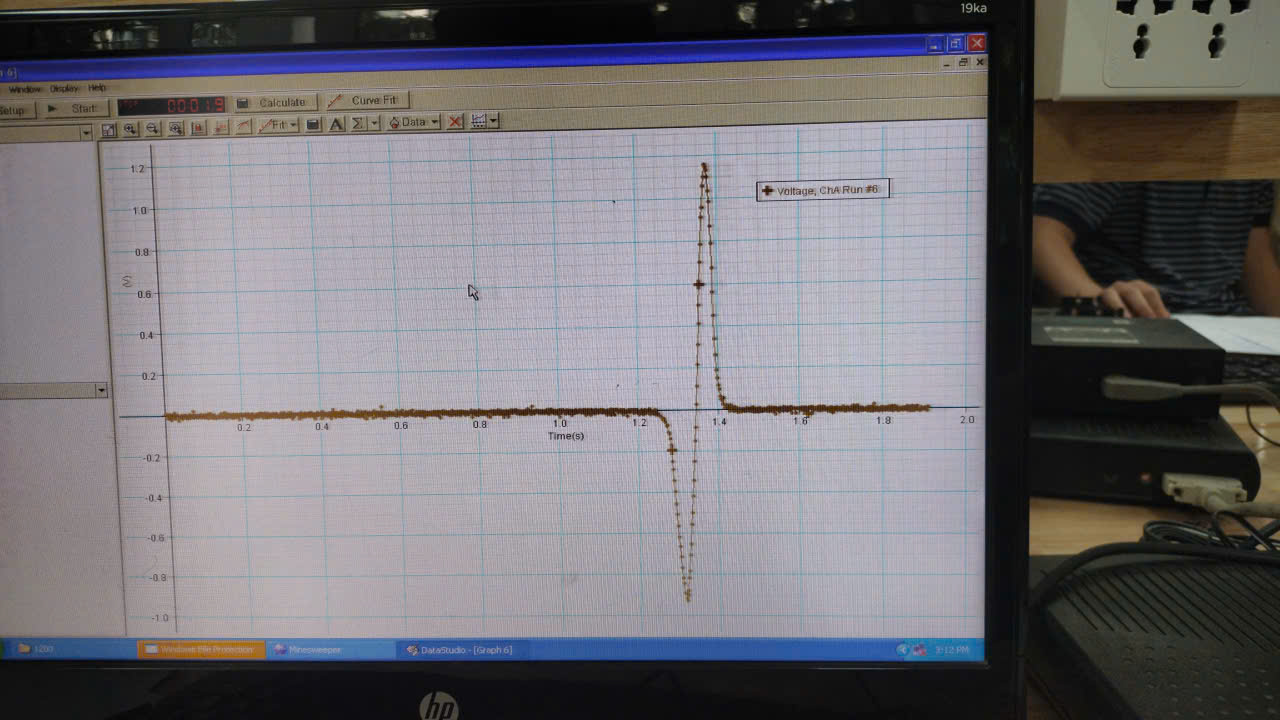
\includegraphics[width=0.95\textwidth]{1200 S.jpg}
		\captionof{figure}{\textit{South-pole down}}
	\end{center}
	
	\begin{center}
		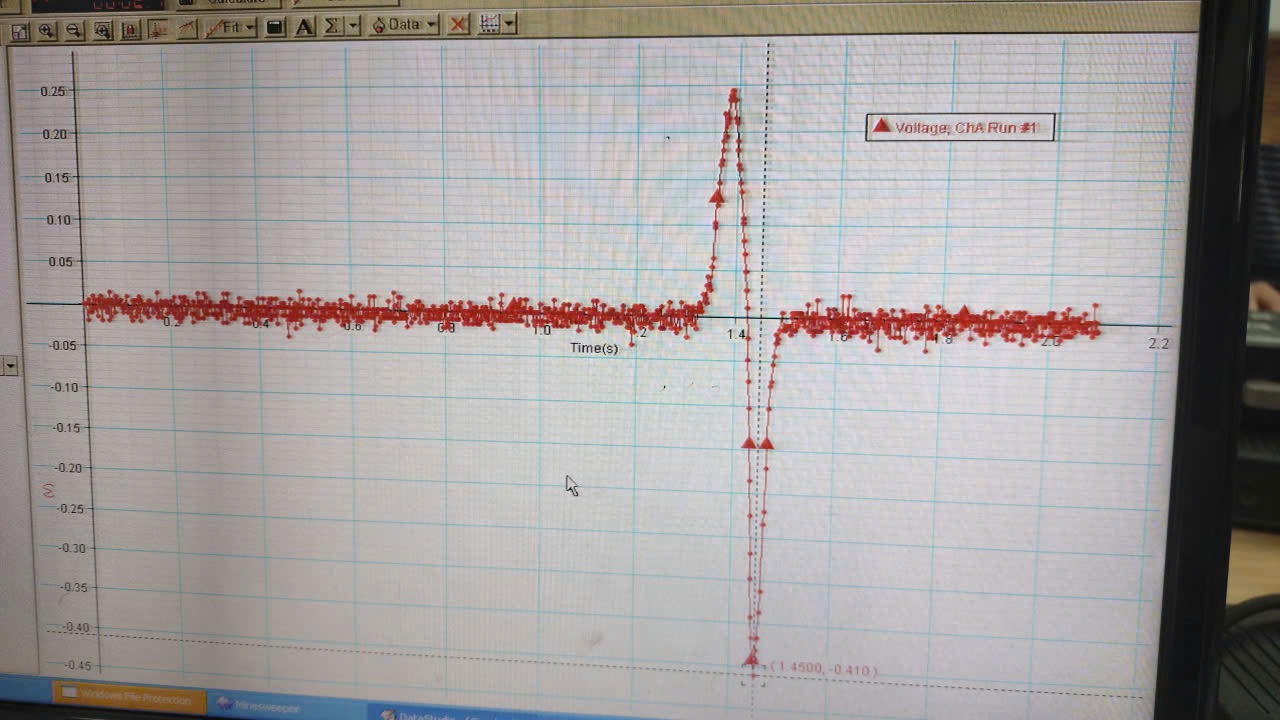
\includegraphics[width=0.95\textwidth]{1200 NS.jpg}
		\captionof{figure}{\textit{North-South combined}}
	\end{center}
	
	\begin{center}
		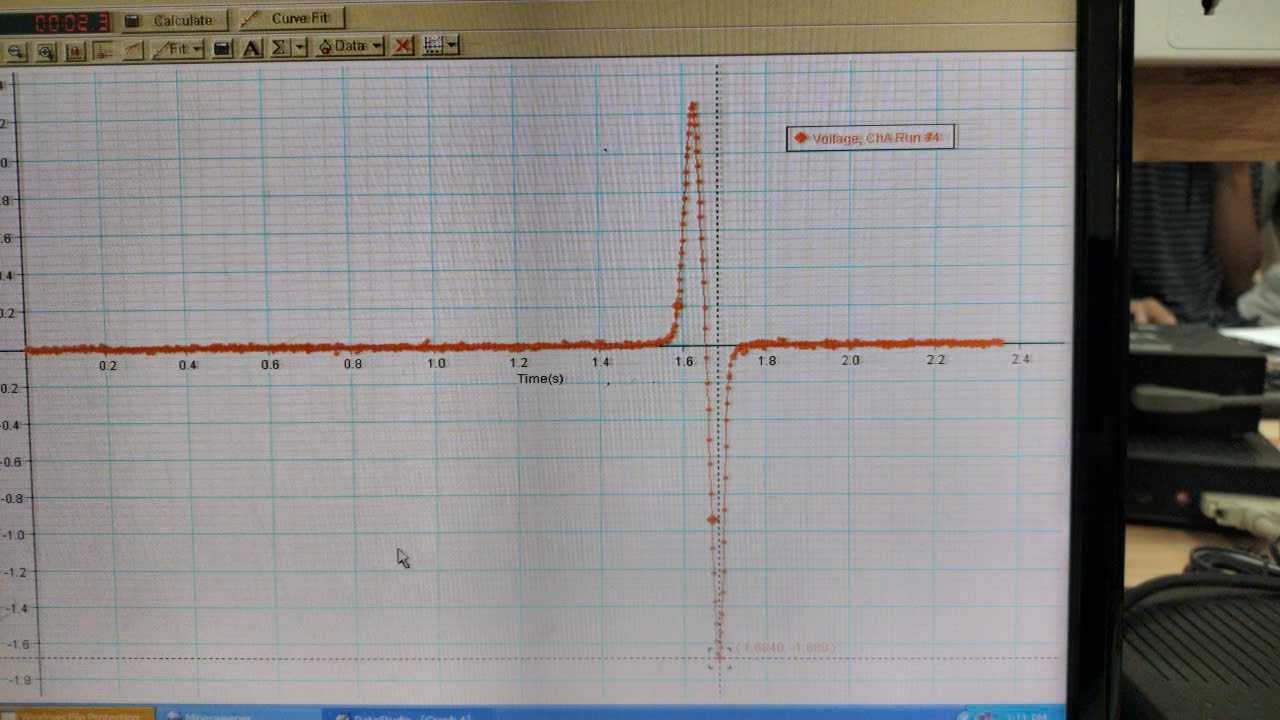
\includegraphics[width=0.95\textwidth]{1200 NN.jpg}
		\captionof{figure}{\textit{North-North down}}
	\end{center}
		
	\subsubsection*{3.1.2. Data Table of Induced Voltage}
	\begin{table}[H]
		\centering
		\caption{Measurement results for 1200-turn coil}
		\begin{tabular}{lccc}
			\toprule
			\textbf{Magnet's pole} & \textbf{Voltage peak 1 (mV)} & \textbf{Voltage peak 2 (mV)} \\
			\midrule
			North pole (N down) & $923$ & $-1187$ \\
			South pole (S down) & $-928$ & $1157$ \\
			Double magnet (N-S combined) & $244$ & $-410$ \\
			Double magnet (N-N / S-S) & $1250$ & $-1680$ \\
			\bottomrule
		\end{tabular}
	\end{table}
	
	\subsection*{3.2. 150-turn coil}
	\subsubsection*{3.2.1. Graph}
	\begin{center}
		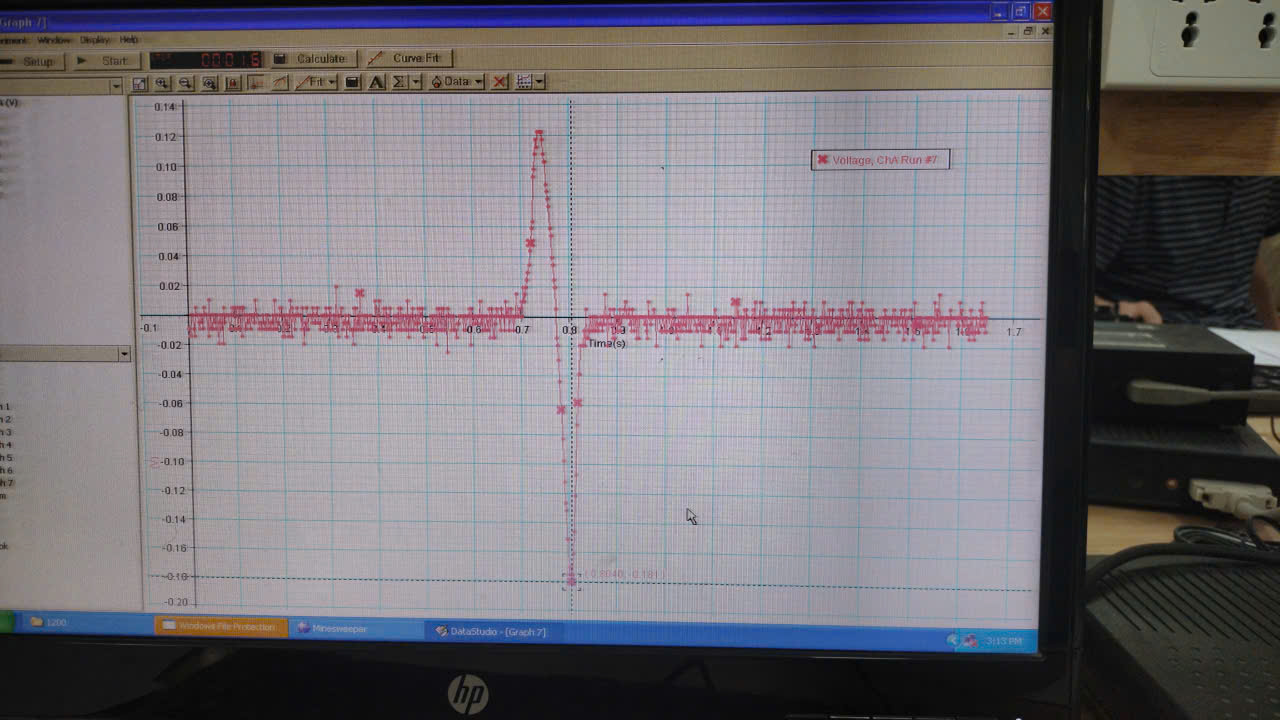
\includegraphics[width=0.95\textwidth]{150 N.jpg}
		\captionof{figure}{\textit{North-pole down}}
	\end{center}
	
	\begin{center}
		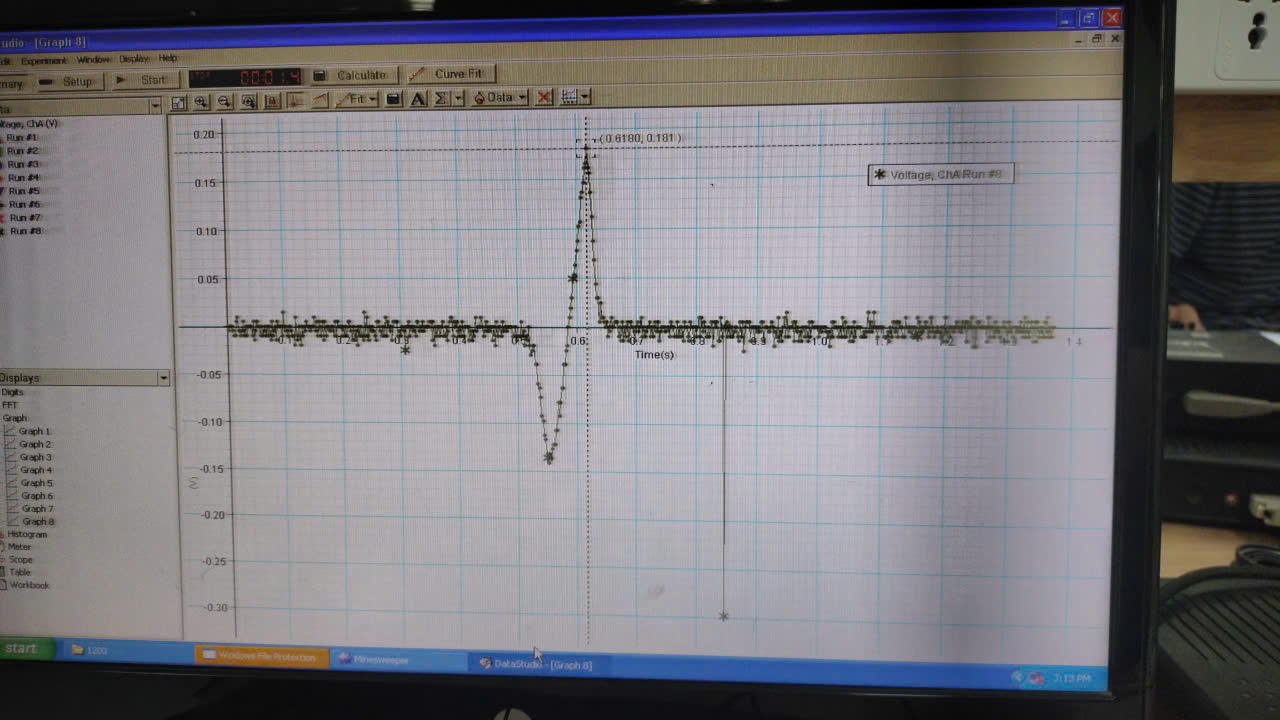
\includegraphics[width=0.95\textwidth]{150 S.jpg}
		\captionof{figure}{\textit{South-pole down}}
	\end{center}
	
	\begin{center}
		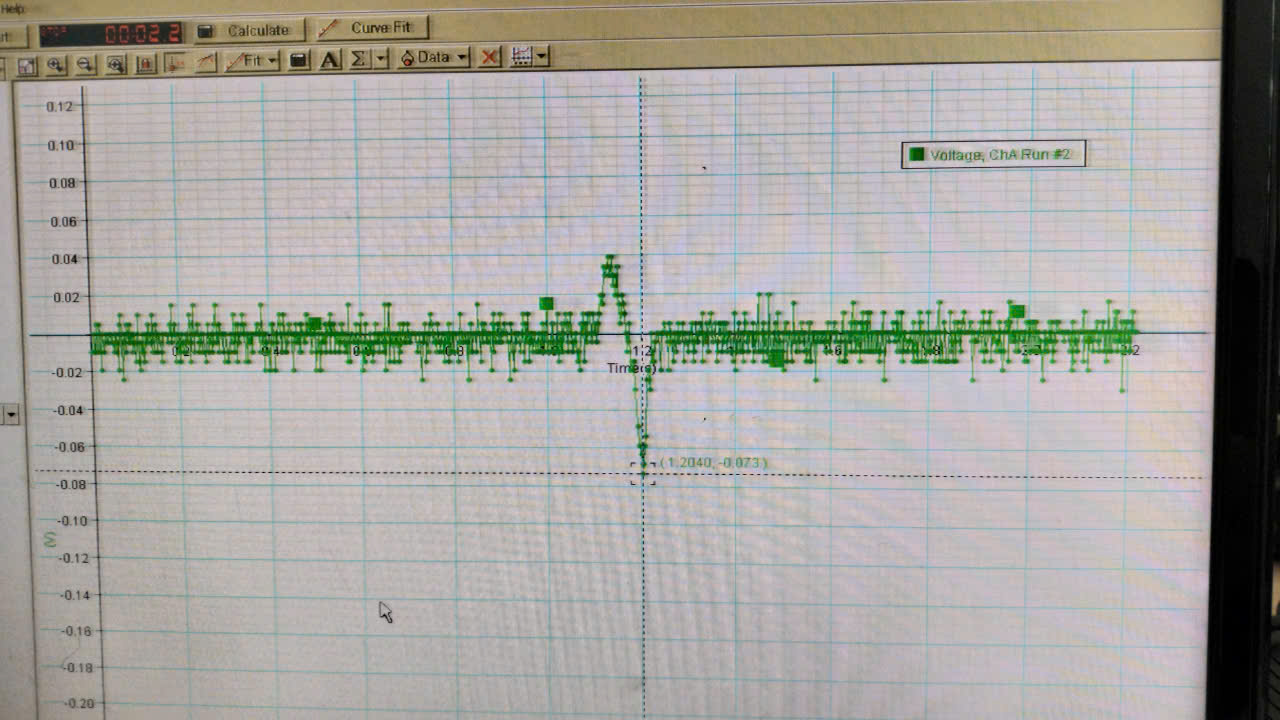
\includegraphics[width=0.95\textwidth]{150 NS.jpg}
		\captionof{figure}{\textit{North-South combined}}
	\end{center}
	
	\begin{center}
		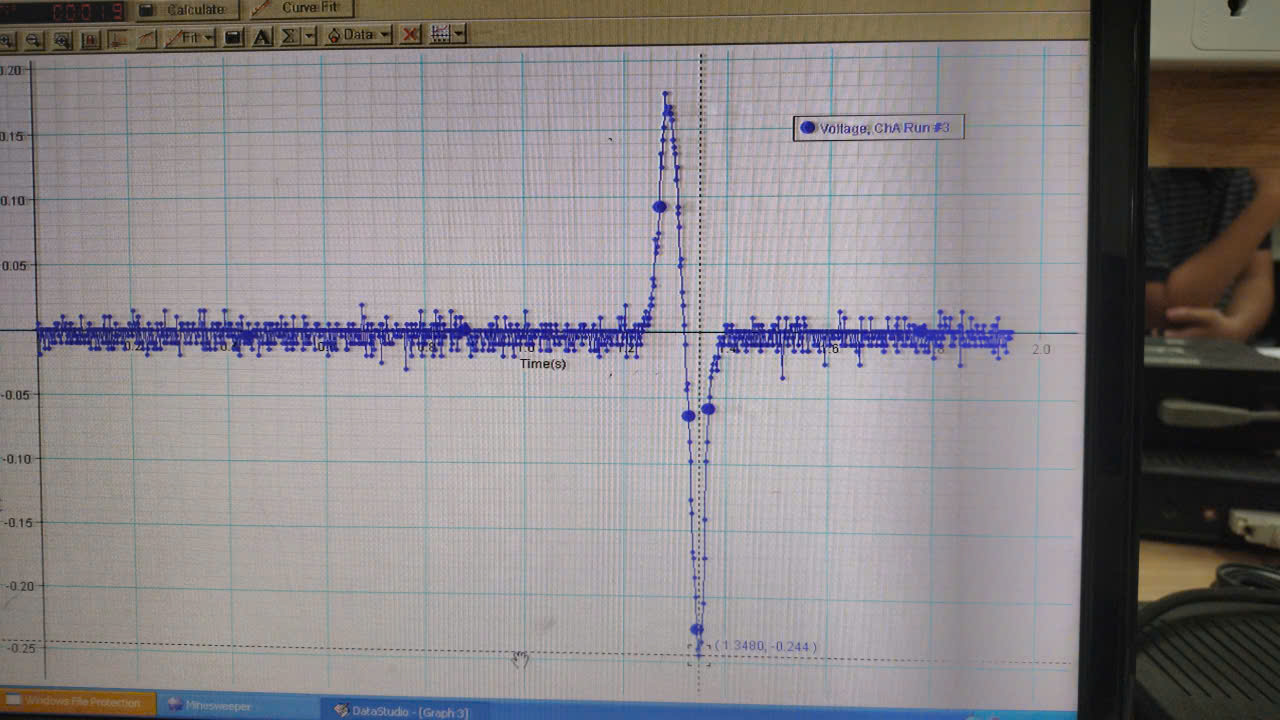
\includegraphics[width=0.95\textwidth]{150 NN.jpg}
		\captionof{figure}{\textit{North-North down}}
	\end{center}
	
	\subsubsection*{3.2.2. Data Table of Induced Voltage}
	\begin{table}[H]
		\centering
		\caption{Measurement results for 150-turn coil}
		\begin{tabular}{lccc}
			\toprule
			\textbf{Magnet's pole} & \textbf{Voltage peak 1 (mV)} & \textbf{Voltage peak 2 (mV)} \\
			\midrule
			North pole (N down) & $122$ & $-181$ \\
			South pole (S down) & $-142$ & $181$ \\
			Double magnet (N-S combined) & $39$ & $-73$ \\
			Double magnet (N-N / S-S) & $176$ & $-244$ \\
			\bottomrule
		\end{tabular}
	\end{table}
	
	\section*{IV. COMMENTS AND EXPLANATIONS}
	
	\begin{bt}
		\textbf{Why is the value of the first voltage peak smaller than that of the second voltage peak?}
		
		When the magnet bar is falling, the gravity acts on it with an acceleration g. Neglecting the air resistance, we have the velocity formula
		\begin{equation}
			v\left(t\right)\approx v_0+gt\approx gt
		\end{equation}
		\qquad Let $t_1$ be the time the magnet bar just enters the coil, and $t_2$ be the time the magnet just leaves the coil. Obviously, we have
		\begin{equation}
			t_1\ <\ t_2\Longrightarrow \left(t_1\right)\ <\ v\left(t_2\right)\Longrightarrow\left|\Delta B_1\right|<\left|\Delta B_2\right|\Longrightarrow\left|V_1\right|=\left|-N\frac{\Delta B_1A}{\Delta t}\right|<\left|-N\frac{\Delta B_2A}{\Delta t}\right|=\left|V_2\right|
		\end{equation}
		where $\Delta B_1\ \text{\ and\ }\ \Delta B_2$ are the changes in the magnetic field when the magnet bar just enters and leaves the coil, respectively. Hence, we can conclude that the value of the first voltage peak is smaller than that of the second voltage peak.
		
	\end{bt}
	
	\begin{bt}
		\textbf{Why are the signals of the induced voltage in the case of N-pole and S-pole inverse with each other?}
		
		Outside the magnet, magnetic field lines travel from the North pole to the South pole. When we flip the magnet (S-pole down), the direction of the magnetic field passing through the coil is inverted compared to the N-pole case. As a result, the direction of the induced current and the polarity of the induced voltage are reversed. Hence, the voltage signals for the N-pole and S-pole cases are opposite to each other.
	\end{bt}
	
	\begin{bt}
		\textbf{Why is the signal produced by the 1200-turn coil larger than that by the 150-turn coil?}
		
	According to Faraday's law of electromagnetic induction, the magnitude of the induced voltage is proportional to the number of turns in the coil.
	In each case (N-pole down, S-pole down, etc.), suppose that the rate of change of magnetic flux  $\frac{\Delta\Phi}{\Delta\ t}$  is the same, we have
	\begin{equation}
		\left|V_{induced}^{1200-turn\ coil}\right|\ =\ \left|-1200\ \frac{\Delta\Phi}{\Delta t}\right|>\left|-150\ \frac{\Delta\Phi}{\Delta t}\right|=\left|V_{induced}^{150-turn\ coil}\right|
	\end{equation}
	
	Therefore, the signal produced by a 1200-turn coil is larger than that by a 150-turn coil.

	\end{bt}
	
	\begin{bt}
		\textbf{What is your comment for the case when you use the set of two magnets for the measurement performed at step 7 and 8?}
		
		 Step 7 (Opposite poles aligned): The magnetic fields of both magnet bars cancel each other out, making the net flux change close to zero. As a result, the induced voltage is nearly zero.
		
		Step 8 (Same poles aligned): Roughly doubles the magnetic field strength, thereby roughly doubling the rate of change of flux and doubling the peak induced voltage.
		
	\end{bt}
	
\end{document}